\chapter{Preliminaries}

\section{Cellular Automata}

A cellular automaton (CA) is a regular lattice of computational units called cells. Each cell $v$ is characterised by a state variable $S_i(t) \in \Sigma$, where $i$ indicates the position of the cell in the lattice and $t$ indicates the time. Each cell also has a finite local neighbourhood set $\mathcal{N}(v)$ with cardinality $N$. Typically, the neighbourhood of a cell contains the cell itself (i.e. $v \in \mathcal{N}(v)$). At each time step, the state of every cell is simultaneously updated according to a fixed transition rule; $\phi:\Sigma^N \to \Sigma$ which takes the neighbour states as input. This rule is typically shared across all cells in the CA.

\subsection{Classification}

The choice of lattice geometry, neighbourhood function, state variable, and transition rule define the behaviour of a CA. Fixing the former three factors, Wolfram \cite{wolfram1986theory} has classified CAs based on transition rules as follows:
\begin{enumerate}
  \item Class 1 (Null) : Rules that lead to a trivial, uniform state
  \item Class 2 (Fixed point + periodic) : Rules that lead to stable or periodic patterns
  \item Class 3 (Chaotic) : Rules that lead to chaotic patterns
  \item Class 4 (Complex) : Rules that lead to complex, long-lived transient patterns
\end{enumerate}

\textbf{Elementary cellular automata} are defined on the simplest nontrivial lattice, a finite one-dimensional chain. The neighbourhood of each cell contains the cell itself and the two cells adjacent to it on either side. The state variable is a boolean which means there are $2^3 = 8$ possible neighbourhood state configurations and $2^8 = 256$ possible transition rules. Each rule can be represented as an 8-digit binary rule table $(t_7t_6t_5t_4t_3t_2t_1t_0)$ where configuration $(000)$ maps to $t_0$, $(001)$ maps to $t_1$, ..., and $(111)$ maps to $(t_7)$. Figure \ref{fig:rule-space} illustrates the distribution of classes in this rule space as we vary $p$, the proportion of 1s in the rule table. \\

The Wolfram code, a number between 0 and 255 obtained by converting the binary rule table to decimal, is the standard naming convention for these rules. Rule 110 is particularly notable as it can exhibit class 4 behaviour \cite{wolfram2002} and has been proven to be Turing Complete \cite{cook2004universality}. Figure \ref{fig:rule-110} shows an example progression of a Rule 110 system. Each row of pixels represents the state of the automaton at one snapshot in time with the topmost row representing the randomized initial state. It shows the emergence, interaction, and subsequent dissipation of multiple long-lived transient patterns.

\begin{figure}[!h]
\centering
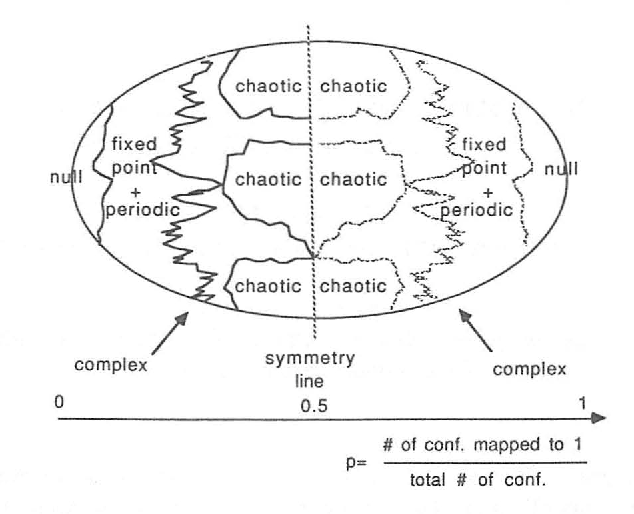
\includegraphics[width=0.9\textwidth]{preliminaries/rule-space.png}
\caption{Schematic illustration of elementary CA rule space from Li and Packard \cite{li1990structure}}
\label{fig:rule-space}
\end{figure}

\begin{figure}[!h]
\centering
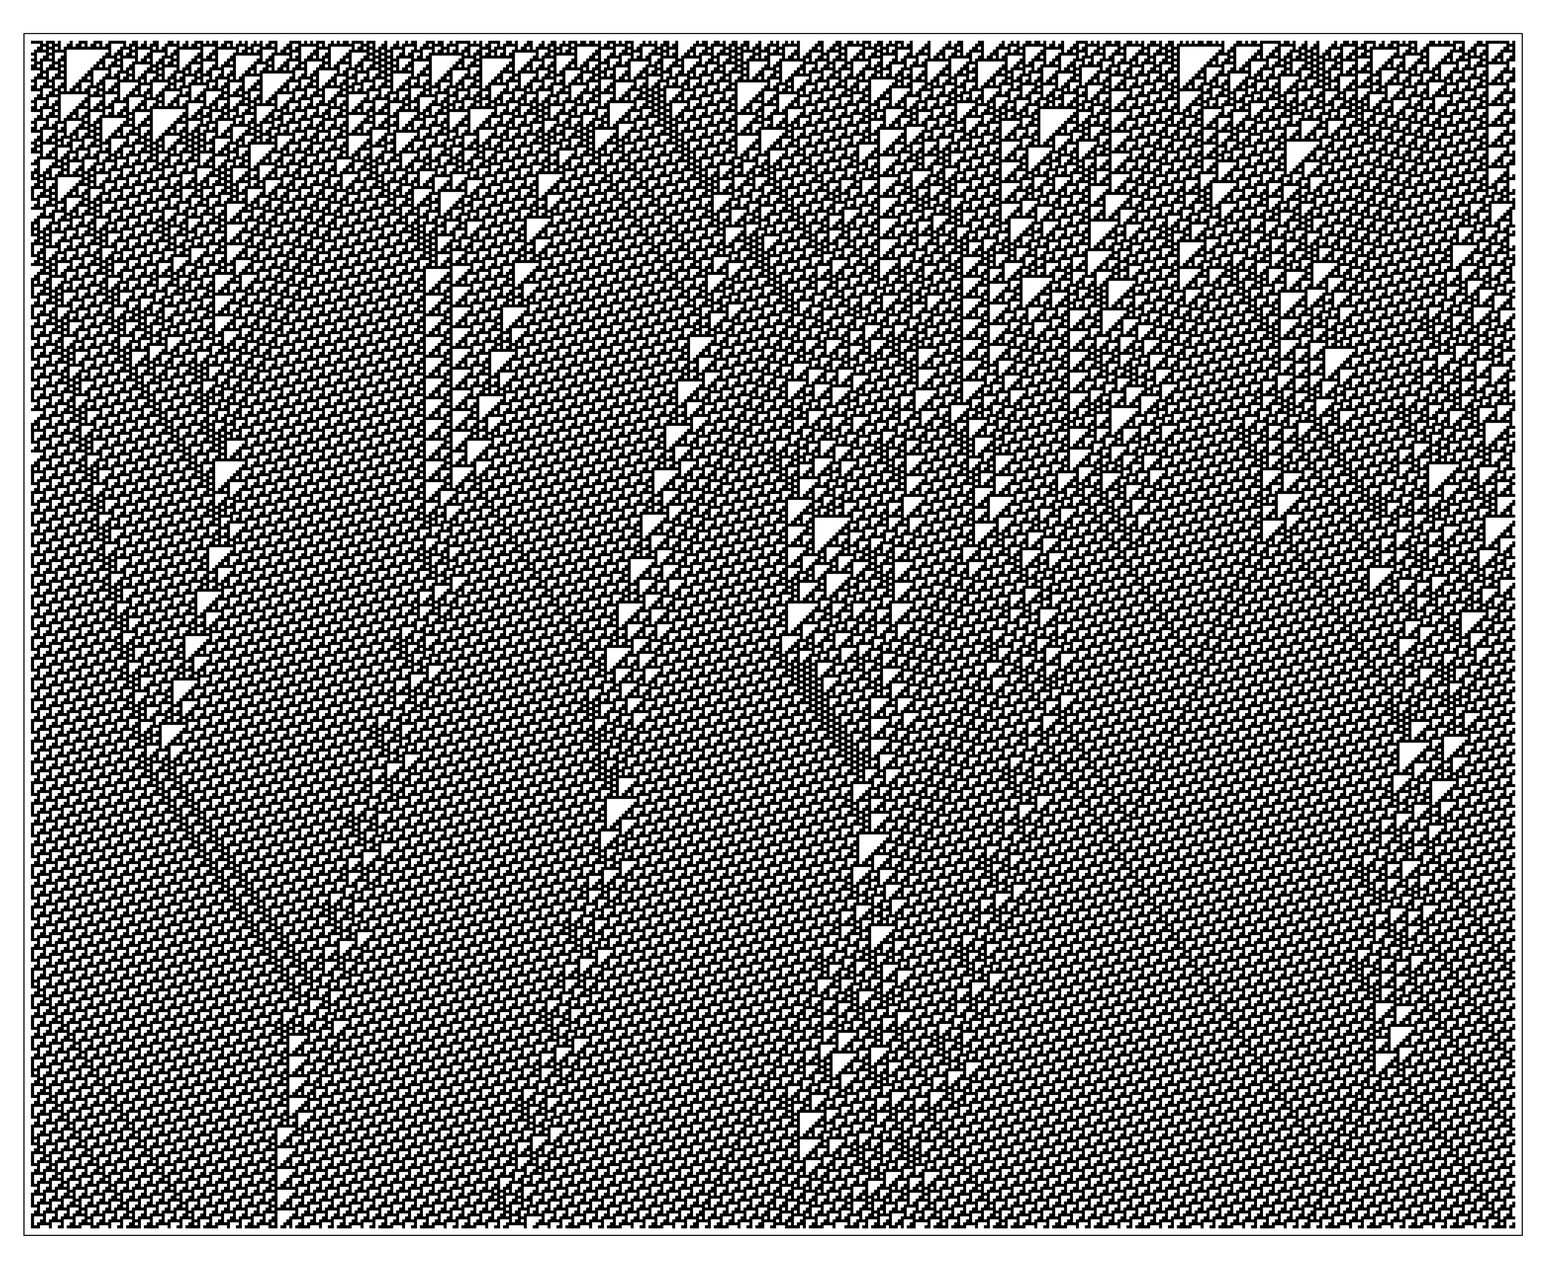
\includegraphics[width=0.9\textwidth]{preliminaries/rule-110.png}
\caption{Rule 110 progression with random initialisation \cite{wolfram2002}}
\label{fig:rule-110}
\end{figure}

\subsection{Morphogenesis}
Morphogenesis is the process by which a system develops into a particular shape or pattern. 
Biologically, this is seen in most multicellular organisms which can robustly develop specialised organs and intricate skin patterns without any centralised decision-making.
Through simple rules encoded in the genome and homeostatic feedback loops enforced through chemical signalling, a tissue knows exactly how to grow and when to stop.\\

Emulating this behaviour \textit{in silico} can provide great insight into the way self-organising and self-repairing biological systems function.
Cellular automata are a promising model of computation for artificial life simulation because, much like biological agents, their behaviour follows logically from combining information in their surroundings and internal programming.
In the context of morphogenesis, we are interested in rules that form fixed point class 2 patterns from random initial conditions. 
We're also interested in rules that are resistant to noise.
Such rules can be thought of as "attractive" solutions in the rule space.

\section{Neural Networks}
Artificial neural network models have proven to be a promising method of learning transition rules for cellular automata. A simple example of such a network is a multilayer perceptron. This is a 3 layered neural network featuring an input layer, a hidden layer with a nonlinear activation function, and an output layer. By the universal approximation theorem, any continuous, bounded function can be approximated arbitrarily well by multilayer perceptron (MLP) \todo{cite}. This section explores different categories of neural networks that have been used to learn transition rules for various cellular automata.

\subsection{Convolutional Neural Networks}
A convolutional neural network is an ANN that is particularly well-suited to inputs in grid-based topologies such as images and videos.
Instead of containing fully connected layers, the neurons in the hidden layers of a CNN only take input from a particular receptive field.
This design decision is broadly inspired by the way biological vision systems work.
Cortical neurons respond only to light hitting a subset of the visual field and there is major overlap between the receptive fields of these neurons.\\

A CNN architecture typically features two broad stages, embedding and classification. 
The embedding stage features convolution, activation, and pooling operations.
The classification stage usually contains fully connected layers.
We will explore the characteristics and purpose of each of these layers in turn.\\

Convolution layers apply a dot product between a shared kernel matrix and a sub-grid of the input. 
The kernel filter slides all such sub-grids and applies the convolution operation to produce an activation map.
An activation function is then applied to each pixel in the activation map to introduce nonlinearity.
Examples include the Sigmoid, Tanh, and ReLU functions.\\

Pooling layers extract key information from sub-grids. Typical pooling operations include max-pooling, average-pooling, and L2 norm pooling. Each one extracts a single value from a kernel filter.\\

\subsection{Graph Neural Networks}


\subsection{Recurrent Neural Networks}

\section{Mesh Construction}